\documentclass{article}
\usepackage[T1]{fontenc}
\usepackage{lmodern}
\usepackage{graphicx}
\usepackage{amsmath,amssymb}
\usepackage[a4paper,margin=2cm]{geometry}
\usepackage[absolute,overlay]{textpos}
\setlength{\TPHorizModule}{1mm}
\setlength{\TPVertModule}{1mm}
\usepackage[indonesian]{babel}
\usepackage{hyperref}
\setlength{\emergencystretch}{2em}
% unit: Halaman 41

\begin{document}

% === Halaman 41 (llm) ===

\section*{Citra Digital}

\vspace{117.91mm}

\begin{itemize}
    \item Citra terdiri dari sejumlah \textit{pixel}. Citra $1200 \times 1500$ berarti memiliki $1200 \times 1500 \text{ pixel} = 1.800.000 \text{ pixel}$
\end{itemize}

\vspace{60mm}

\begin{itemize}
    \item Setiap \textit{pixel} panjangnya $n$-bit.
    \begin{itemize}
        \item Citra biner $\rightarrow 1 \text{ bit/pixel}$
        \item Citra \textit{grayscale} $\rightarrow 8 \text{ bit/pixel}$
        \item Citra \textit{true color} $\rightarrow 24 \text{ bit/pixel}$
    \end{itemize}
\end{itemize}

% deskripsi: Foto Taj Mahal sebagai contoh citra digital asli.
% bbox normalisasi: [0.1790, 0.2760, 0.4110, 0.6730]
\begin{textblock*}{48.72mm}(37.59mm,81.97mm)
\noindent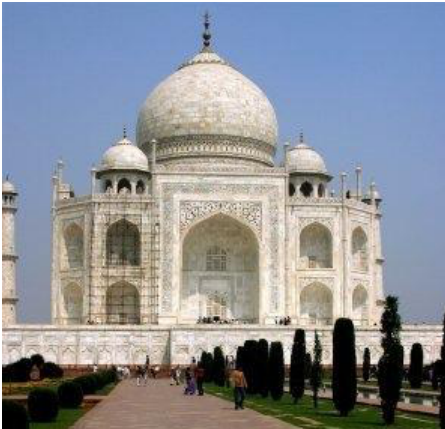
\includegraphics[width=48.72mm,height=117.91mm]{../../images/llm/page_041_img_01.png}%
\end{textblock*}

% deskripsi: Foto Taj Mahal dengan overlay grid yang mengilustrasikan konsep pixel pada citra digital.
% bbox normalisasi: [0.5110, 0.2670, 0.8310, 0.6980]
\begin{textblock*}{67.20mm}(107.31mm,79.30mm)
\noindent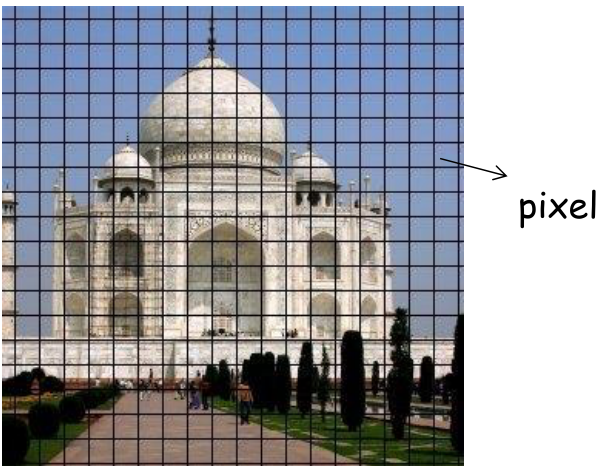
\includegraphics[width=67.20mm,height=128.01mm]{../../images/llm/page_041_img_02.png}%
\end{textblock*}

\end{document}
